\documentclass[letterpaper,12pt]{article}
\usepackage[bottom=2.5cm, top=2.5cm, right=2cm, left=3cm]{geometry}
\usepackage[spanish, es-tabla]{babel}
\usepackage{graphicx} 
\usepackage{hyperref}
\usepackage{booktabs}
\usepackage{natbib}
\usepackage{float}
\usepackage{listings}
\usepackage{xcolor}
\usepackage{parskip} 
\usepackage{fancyhdr} % Paquete para personalizar encabezados y pies de página
\usepackage{microtype}  % Mejora la justificación del texto
\usepackage{amsmath}


% Definición de colores al estilo Visual Studio Code
\definecolor{codegreen}{rgb}{0.25,0.49,0.48} % Comentarios
\definecolor{codegray}{rgb}{0.5,0.5,0.5} % Números y anotaciones
\definecolor{codepurple}{rgb}{0.58,0,0.82} % Palabras clave
\definecolor{backcolour}{rgb}{0.95,0.95,0.92} % Color de fondo

% Configuración del estilo de las celdas de código
\lstset{
    backgroundcolor=\color{backcolour},   % color de fondo; necesita que el paquete color o xcolor esté cargado
    commentstyle=\color{codegreen},       % estilo de comentarios
    keywordstyle=\color{codepurple},      % estilo de palabras clave
    numberstyle=\tiny\color{codegray},    % estilo de los números de línea
    stringstyle=\color{red},              % estilo de las cadenas de texto
    basicstyle=\ttfamily\small,           % estilo del texto básico
    breakatwhitespace=false,              % ajustes de líneas sólo en espacios en blanco
    breaklines=true,                      % ajustar las líneas si son muy largas
    captionpos=b,                         % posición de la leyenda (abajo)
    keepspaces=true,                      % preserva los espacios en el texto; útil si se usa monoespaciado
    numbers=left,                         % dónde poner los números de línea
    numbersep=5pt,                        % qué tan lejos están los números de línea del código
    showspaces=false,                     % mostrar espacios con subrayados particulares; reemplaza 'showstringspaces'
    showstringspaces=false,               % subrayar los espacios dentro de las cadenas solo
    showtabs=false,                       % mostrar tabulaciones en el código con subrayados particulares
    tabsize=2,                            % tamaños de tabulación a 2 espacios
    language=TeX,                         % lenguaje del código
    morecomment=[l]\#,                    % reconocer # como inicio de comentario en Python
    frame=single,                         % agregar un marco simple alrededor del código
    rulecolor=\color{black}               % color del marco
}
\hypersetup{
    colorlinks=true,
    linkcolor=black,
    citecolor=black,
    urlcolor=blue
}

% Configuración del encabezado
\pagestyle{fancy}
\fancyhf{} % Limpia los encabezados y pies de página actuales
\fancyhead[R]{\thepage} % Coloca el número de página en la parte superior derecha
\renewcommand{\headrulewidth}{0pt} % Elimina la línea horizontal en la parte superior de la página

\begin{document}

\begin{titlepage}
    \begin{center}
      \vspace*{1cm}

    \textbf{\Large DISTRIBUCIÓN DE VIAJES EN SAN CARLOS DE APOQUINDO}
    
    \vspace{1cm}
    
    \textbf{Bernardo Caprile Canala-Echevarría y Pedro Tomás Valenzuela Bejares}\\
    Facultad de Ingeniería y Ciencias Aplicadas, Universidad de los Andes, Santiago de Chile\\
    e-mail: \href{mailto:bcaprile@miuandes.cl}{bcaprile@miuandes.cl}, \href{mailto: ptvalenzuela@miuandes.cl}{ptvalenzuela@miuandes.cl}
    
    \vspace{2cm}
    
    \textbf{RESUMEN}
    
     
    \end{center}
    El presente informe aborda la distribución de viajes en San Carlos de Apoquindo utilizando matrices origen-destino, generadas mediante el modelo gravitacional y el método de Furness. En primer lugar, se obtuvo una matriz inicial con el modelo gravitacional, utilizando datos de origen-destino y una función de costos. Posteriormente, para mejorar la precisión y ajustar los totales de viajes, se aplicó el método de Furness, el cual permitió equilibrar la matriz iterativamente. Se observó que las zonas E1, E2, E3 y E4 presentaron las mayores diferencias, tanto antes como después del ajuste, debido a que el método iterativo busca alinear la matriz con los valores esperados para 2024. Los resultados indican que, aunque estos métodos son efectivos para modelar la distribución de viajes, presentan limitaciones, ya que no capturan ciertos factores como la congestión o cambios en infraestructura y transporte. Finalmente, se concluye que la matriz modelada para 2024 ofrece una aproximación coherente, pero puede diferir de la realidad debido a factores imprevistos.

    \vspace{0.5cm} 
    \textit{Palabras clave:} Matriz origen-destino, método de Furness, modelo gravitacional, distribución de viajes, San Carlos de Apoquindo.
\end{titlepage}

\newpage

\section{Introducción}

El flujo de vehículos en hora punta de la mañana en San Carlos de Apoquindo es un problema significativo, ya que esta zona, además de ser un barrio residencial, se caracteriza por tener una alta concentración de colegios y universidades. Por lo tanto, el tráfico matutino afecta tanto a los residentes que salen como a los estudiantes que ingresan a esta área. Para poder tomar decisiones respecto al flujo vehicular, no solo en San Carlos de Apoquindo, sino en todo Santiago, se realiza periódicamente la encuesta origen-destino, la cual permite conocer la cantidad de viajes que se realizan en la ciudad y su distribución.

Con esta información, se pueden generar modelos y tomar decisiones, las cuales optimicen las rutas de las personas, disminuyendo el tráfico y el tiempo de viaje. Por esta razón, es importante contar con una matriz origen-destino actualizada y precisa, la cual permita realizar análisis y proyecciones de la distribución de viajes en la ciudad. A continuación, se presenta la figura \ref{fig:mapa}, la cual muestra la zonificación de una parte de Las Condes enfocada en San Carlos de Apoquindo. 

\begin{figure}[h!]
    \centering
    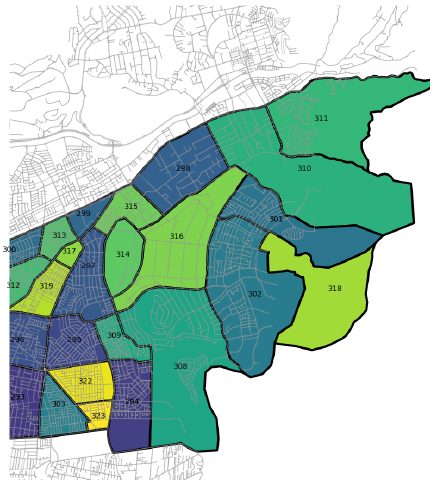
\includegraphics[width=0.5\textwidth]{fotos/mapa.png}
    \caption{Mapa de San Carlos de Apoquindo.}
    \label{fig:mapa}
\end{figure}

Para esta tarea, se generarán 3 matrices origen-destino en base a esta zonificación mediante un código Python: La primera ocupando un modelo gravitacional con una matriz de costos, como distancia de viaje promedio, luego se le aplicará el método de Furness con vectores del 2024. Finalmente, se calibrará la matriz minimizando el error cuadrático medio y se compararán los resultados obtenidos.



\section{Resultados y Discusiones}
Los cálculos se realizaron en Python, utilizando las librerías Pandas y Numpy. El código se encuentra en el repositorio de GitHub \href{https://github.com/berckanala/T3_autitos/blob/main/t3.py}{Código}
\subsection{Matriz Origen-Destino con el Modelo Gravitacional}
Primero, se generó una Matriz Origen-Destino utilizando el modelo gravitacional, aplicando la ecuación \ref{eq} proporcionada junto con la matriz de costos entre zonas (Tabla \ref{table:costs_zones}) y los vectores de origen y destino de 2012 (Tabla \ref{table:oi_dj_2012}).

\begin{equation}
    T_{ij} = \alpha \cdot O_{i,2012} \cdot D_{j,2012} \cdot C_{ij}^k \cdot e^{-\beta \cdot C_{ij}}
    \label{eq}
\end{equation}

Donde:
\begin{itemize}
    \item $T_{ij}$ es la cantidad de viajes entre la zona $i$ y la zona $j$.
    \item $O_{i,2012}$ es la cantidad de viajes de origen en la zona $i$.
    \item $D_{j,2012}$ es la cantidad de viajes de destino en la zona $j$.
    \item $C_{ij}$ es el costo entre la zona $i$ y la zona $j$.
    \item $\alpha$ y $k$ son parámetros a calibrar.
    \item $\beta$ es un parámetro equivalente a 0.2176.
\end{itemize}



Con todos los valores se procede a calcular el parámetro $\alpha$ con un k igual a 1. Para ello, se ocupó la siguiente ecuación:

\begin{equation}
    \alpha = \frac{\sum_i O_{i,2012}}{\sum_i \sum_j O_{i,2012} \cdot D_{j,2012} \cdot C_{ij}^k \cdot e^{-\beta \cdot C_{ij}}}
    \label{eq:alpha}
\end{equation}

Luego de aplicar la ecuación \ref{eq:alpha}, se obtuvo un  $\alpha$ igual a $3.249 \cdot 10^{-5}$, con el cual se procedió a calcular la matriz de viajes que se muestra a continuación:


\begin{table}[H]
    \centering
    \resizebox{\textwidth}{!}{%
    \begin{tabular}{c|ccccccccccc}    
    \textbf{Zona O\textbackslash D} & \textbf{301} & \textbf{302} & \textbf{308} & \textbf{314} & \textbf{316} & \textbf{318} & \textbf{E1} & \textbf{E2} & \textbf{E3} & \textbf{E4} & \textbf{Oi,2024} \\ \hline
    \textbf{301} & 64.1 & 849.2 & 243.6 & 232.3 & 120.1 & 57.9 & 196.3 & 102.6 & 266.5 & 191.7 & 2324.3 \\ 
    \textbf{302} & 556.4 & 2127.7 & 1047.0 & 633.0 & 306.5 & 276.8 & 651.7 & 310.3 & 961.7 & 727.7 & 7598.8 \\ 
    \textbf{308} & 412.0 & 2702.6 & 555.9 & 471.3 & 281.3 & 326.2 & 556.8 & 249.5 & 880.2 & 727.1 & 7163.1 \\ 
    \textbf{314} & 2.9 & 12.0 & 3.5 & 1.1 & 1.1 & 1.8 & 3.2 & 1.3 & 4.1 & 3.8 & 34.6 \\ 
    \textbf{316} & 236.9 & 922.7 & 328.1 & 169.3 & 84.7 & 145.8 & 290.6 & 124.0 & 368.6 & 312.2 & 2982.8 \\ 
    \textbf{318} & 0.0 & 0.3 & 0.2 & 0.1 & 0.1 & 0.0 & 0.1 & 0.1 & 0.1 & 0.1 & 1.1 \\ 
    \textbf{E1} & 118.8 & 601.8 & 199.2 & 158.2 & 89.1 & 73.2 & 0.0 & 0.0 & 0.0 & 0.0 & 1240.3 \\ 
    \textbf{E2} & 124.5 & 574.8 & 179.1 & 126.3 & 76.3 & 75.0 & 0.0 & 0.0 & 0.0 & 0.0 & 1155.9 \\ 
    \textbf{E3} & 767.0 & 4225.4 & 1498.2 & 946.0 & 538.0 & 468.6 & 0.0 & 0.0 & 0.0 & 0.0 & 8443.1 \\ 
    \textbf{E4} & 298.3 & 1728.2 & 669.0 & 471.1 & 246.3 & 190.9 & 0.0 & 0.0 & 0.0 & 0.0 & 3603.9 \\ \hline
    \textbf{Dj, 2024} & 2580.9 & 13744.7 & 4723.6 & 3208.8 & 1743.5 & 1616.2 & 1698.8 & 787.8 & 2481.1 & 1962.6 & 34548.0 \\
    \end{tabular}}
    \caption{Matriz Origen-Destino con método global}
    \label{table:global}
  \end{table}
  

\subsection{Implementación del Método Furness}
Para poder mejorar la presición de la matriz obtenida (Tabla \ref{table:global}), se implementó el método Furness, este método es un algoritmo iterativo que equilibra la matriz de viajes para que las sumas de sus columnas y filas coincidan con los totales proyectados, manteniendo la distribución proporcional de los viajes según una matriz base. A continuación se muestra la matriz obtenida:
\begin{table}[H]
    \centering
    \resizebox{\textwidth}{!}{%
    \begin{tabular}{c|ccccccccccc}    
    \textbf{Zona O\textbackslash D} & \textbf{301} & \textbf{302} & \textbf{308} & \textbf{314} & \textbf{316} & \textbf{318} & \textbf{E1} & \textbf{E2} & \textbf{E3} & \textbf{E4} & \textbf{Oi,2024} \\ \hline
    \textbf{301} & 31.4 & 147.7 & 51.5 & 25.1 & 45.4 & 16.4 & 314.3 & 128.9 & 361.2 & 622.1 & 1744.0 \\ 
    \textbf{302} & 251.1 & 341.0 & 204.0 & 63.0 & 106.8 & 72.1 & 961.5 & 359.3 & 1201.4 & 2175.7 & 5736.0 \\ 
    \textbf{308} & 173.9 & 405.0 & 101.3 & 43.8 & 91.7 & 79.5 & 768.2 & 270.2 & 1028.3 & 2033.1 & 4995.0 \\ 
    \textbf{314} & 0.9 & 1.4 & 0.5 & 0.1 & 0.3 & 0.3 & 3.5 & 1.1 & 3.7 & 8.2 & 20.0 \\ 
    \textbf{316} & 103.8 & 143.6 & 62.1 & 16.4 & 28.7 & 36.9 & 416.4 & 139.4 & 447.2 & 906.6 & 2301.0 \\ 
    \textbf{318} & 0.0 & 0.1 & 0.0 & 0.0 & 0.0 & 0.0 & 0.2 & 0.1 & 0.2 & 0.4 & 1.0 \\ 
    \textbf{E1} & 671.5 & 1208.0 & 486.2 & 197.1 & 389.2 & 238.9 & 0.0 & 0.0 & 0.0 & 0.0 & 3191.0 \\ 
    \textbf{E2} & 542.8 & 889.9 & 337.2 & 121.4 & 256.9 & 188.8 & 0.0 & 0.0 & 0.0 & 0.0 & 2337.0 \\ 
    \textbf{E3} & 3069.2 & 6003.3 & 2588.5 & 834.4 & 1662.1 & 1082.5 & 0.0 & 0.0 & 0.0 & 0.0 & 15240.0 \\ 
    \textbf{E4} & 2892.2 & 5949.0 & 2800.6 & 1006.7 & 1844.0 & 1068.5 & 0.0 & 0.0 & 0.0 & 0.0 & 15561.0 \\ \hline
    \textbf{Dj, 2024} & 7737.0 & 15089.0 & 6632.0 & 2308.0 & 4425.0 & 2784.0 & 2464.0 & 899.0 & 3042.0 & 5746.0 & 51126.0 \\
    \end{tabular}}
    \caption{Matriz Origen-Destino con método Furness}
    \label{table:furness}
  \end{table}

\subsubsection{Error Cuadrático Medio}
Luego, se calculó el error cuadrático medio respecto a la original con el siguiente código:


\begin{lstlisting}[language=Python, label={lst:code}]
    mse = np.mean((Tij_df - df1_1) ** 2)
\end{lstlisting}

Donde:
\begin{itemize}
    \item $Tij\_df$ es la matriz de viajes obtenida. (Tabla \ref{table:furness})
    \item $df1\_1$ es la matriz original. (Tabla \ref{table:data_matrix})
\end{itemize}

El error que se obtuvo fue de 350710.81, por lo que, para minimizar el error, se tiene que modificar el k.

\subsection{Calibración de la Matriz Origen-Destino con el Modelo Gravitacional}
Para determinar el valor óptimo de \( k \), se realizaron iteraciones sobre diferentes valores de \( k \), desde 0.001 hasta 10, con incrementos de 0.001, para luego aplicar el error cuadrático \ref{lst:code} hasta encontrar el mínimo. El error mínimo se obtuvo con un \( k \) de 0.001 y un \( \alpha \) de 0.00011, resultando en un error de 345361.66. A continuación, se presenta las matrices resultantes:

\begin{table}[H]
    \centering
    \resizebox{\textwidth}{!}{%
    \begin{tabular}{c|ccccccccccc}    
    \textbf{Zona O\textbackslash D} & \textbf{301} & \textbf{302} & \textbf{308} & \textbf{314} & \textbf{316} & \textbf{318} & \textbf{E1} & \textbf{E2} & \textbf{E3} & \textbf{E4} & \textbf{Oi,2024} \\ \hline
    \textbf{301} & 443.1 & 1588.3 & 550.9 & 258.5 & 187.2 & 259.8 & 70.1 & 69.0 & 104.3 & 41.5 & 3572.7 \\ 
    \textbf{302} & 1040.6 & 5617.8 & 1347.2 & 986.8 & 679.7 & 725.4 & 244.7 & 175.4 & 450.9 & 170.7 & 11439.1 \\ 
    \textbf{308} & 931.6 & 3477.5 & 1538.1 & 900.9 & 537.7 & 488.7 & 213.9 & 128.3 & 504.0 & 185.9 & 8906.6 \\ 
    \textbf{314} & 3.2 & 18.7 & 6.6 & 5.6 & 2.9 & 2.1 & 1.6 & 0.8 & 2.1 & 1.0 & 44.6 \\ 
    \textbf{316} & 369.2 & 2046.2 & 627.1 & 468.3 & 295.8 & 231.4 & 130.1 & 82.9 & 171.9 & 77.1 & 4500.0 \\ 
    \textbf{318} & 0.2 & 0.9 & 0.2 & 0.1 & 0.1 & 0.1 & 0.0 & 0.0 & 0.1 & 0.0 & 1.9 \\ 
    \textbf{E1} & 42.4 & 226.0 & 76.5 & 77.9 & 39.9 & 25.9 & 0.0 & 0.0 & 0.0 & 0.0 & 488.6 \\ 
    \textbf{E2} & 83.7 & 324.8 & 92.0 & 78.9 & 51.0 & 43.5 & 0.0 & 0.0 & 0.0 & 0.0 & 673.9 \\ 
    \textbf{E3} & 300.3 & 1981.0 & 857.8 & 482.0 & 250.9 & 180.2 & 0.0 & 0.0 & 0.0 & 0.0 & 4052.3 \\ 
    \textbf{E4} & 64.6 & 405.4 & 171.0 & 124.5 & 60.8 & 41.8 & 0.0 & 0.0 & 0.0 & 0.0 & 868.2 \\ \hline
    \textbf{Dj, 2024} & 3279.1 & 15686.5 & 5267.5 & 3383.5 & 2106.1 & 1999.1 & 660.4 & 456.3 & 1233.2 & 476.2 & 34548.0 \\
    \end{tabular}}
    \caption{Matriz Origen-Destino con método gravitacional}
    \label{table:calibrada gravitacional}
\end{table}
  

\begin{table}[H]
    \centering
    \resizebox{\textwidth}{!}{%
    \begin{tabular}{c|ccccccccccc}    
    \textbf{Zona O\textbackslash D} & \textbf{301} & \textbf{302} & \textbf{308} & \textbf{314} & \textbf{316} & \textbf{318} & \textbf{E1} & \textbf{E2} & \textbf{E3} & \textbf{E4} & \textbf{Oi,2024} \\ \hline
    \textbf{301} & 121.5 & 142.5 & 53.6 & 13.0 & 34.7 & 41.8 & 301.6 & 155.0 & 298.9 & 581.6 & 1744.0 \\ 
    \textbf{302} & 257.9 & 455.7 & 118.5 & 44.7 & 114.0 & 105.5 & 952.5 & 356.4 & 1168.2 & 2162.6 & 5736.0 \\ 
    \textbf{308} & 205.8 & 251.4 & 120.6 & 36.4 & 80.4 & 63.3 & 742.1 & 232.3 & 1163.7 & 2099.0 & 4995.0 \\ 
    \textbf{314} & 0.5 & 1.0 & 0.4 & 0.2 & 0.3 & 0.2 & 4.2 & 1.1 & 3.6 & 8.5 & 20.0 \\ 
    \textbf{316} & 83.8 & 151.9 & 50.5 & 19.4 & 45.4 & 30.8 & 463.5 & 154.2 & 407.5 & 894.0 & 2301.0 \\ 
    \textbf{318} & 0.1 & 0.1 & 0.0 & 0.0 & 0.0 & 0.0 & 0.2 & 0.1 & 0.2 & 0.3 & 1.0 \\ 
    \textbf{E1} & 676.5 & 1180.1 & 433.5 & 227.2 & 430.8 & 242.8 & 0.0 & 0.0 & 0.0 & 0.0 & 3191.0 \\ 
    \textbf{E2} & 658.3 & 836.0 & 257.0 & 113.4 & 271.4 & 200.8 & 0.0 & 0.0 & 0.0 & 0.0 & 2337.0 \\ 
    \textbf{E3} & 2830.9 & 6111.3 & 2870.6 & 831.0 & 1599.7 & 996.5 & 0.0 & 0.0 & 0.0 & 0.0 & 15240.0 \\ 
    \textbf{E4} & 2901.7 & 5958.9 & 2727.2 & 1022.6 & 1848.3 & 1102.3 & 0.0 & 0.0 & 0.0 & 0.0 & 15561.0 \\ \hline
    \textbf{Dj, 2024} & 7737.0 & 15089.0 & 6632.0 & 2308.0 & 4425.0 & 2784.0 & 2464.0 & 899.0 & 3042.0 & 5746.0 & 51126.0 \\
    \end{tabular}}
    \caption{Matriz Origen-Destino calibrada con método Furness}
    \label{table:calibrada}
  \end{table}
  
\subsection{Discusiones}

Luego de aplicar el método de Furness, la matriz se ajusta para que las sumas de las filas y columnas coincidan con los totales proyectados. Esto genera cambios en la matriz, y se observa en las Tablas \ref{table:calibrada gravitacional} y \ref{table:calibrada} que los viajes entre zonas internas bajan de forma significativa, mientras que los viajes de zonas externas a internas o viceversa aumentan hasta 10 ordenes de magnitud. Esto se debe a que, al ser un método iterativo, es necesario ajustar la matriz para cumplir las restricciones deseadas. Además, al cambiar el valor de $k$, se afectan otras variables como $\alpha$, lo que genera cambios en la función de costos. Un valor de $k$ bajo genera mayor atracción hacia las zonas más cercanas o con un menor costo. En el caso de las zonas mencionadas, E1, E2, E3 y E4, tuvieron que ajustarse significativamente para alinearse con los vectores de destino y origen de 2024. Además, los valores de generación de viajes del cuadrante de los 300 en la Tabla 3 son muy altos y difieren de lo esperado para 2024, por lo que, al aplicar el método de Furness, estos valores disminuyen notablemente y se logran adaptar a lo esperado para 2024, generando una matriz más coherente. Al comparar la matriz original con la final (Tablas \ref{table:data_matrix} y \ref{table:calibrada} respectivamente), se observa que las zonas E1, E2, E3 y E4 siguen siendo las que más difieren respecto a las otras zonas. Esto puede deberse a que, como se mencionó antes, el método de Furness y el modelo gravitacional son ajustes para lograr una representación coherente, pero pueden existir diferencias con la realidad debido a factores que no captura este tipo de modelos.\\

Con respecto a las limitaciones que tiene el metodo de Furness y el modelo gravitacional se puede mencionar que este modelo solo considera ciertos impulsos sobre los viajes como lo son el costo y el tamaño de la zona de origen y destino, lo cual puede no captar otros factores importantes como la congestion, cambios de trasporte publico o privado, entre otros. Ademas, el metodo de Furness ajusta de manera proporcional, lo que puede significar que no se refleje con precision los patrones de viaje o los cambios en este. Luego agregar que los parametros como k, pueden variar en la zona, por lo que no son del todo correctas en cada ocasion. \\

Finalmente, la matriz modelada para 2024 podria diferir de la realidad debido a que no se consideran factores como la pandemia, cambios en la infraestructura, cambios en la densidad poblacional, conflictos sociales, teletrabajo, entre otros. Por lo que se debe tener en cuenta que estos modelos son una aproximacion y no una representacion exacta de la realidad.

\section{Conclusion}

En este trabajo se generaron matrices origen-destino para la zona de San Carlos de Apoquindo, utilizando el método gravitacional y el método Furness. Se obtuvo una matriz calibrada con el método gravitacional y se comparó con la matriz original, obteniendo un error cuadrático medio de 345361.66. Se concluye que el método Furness es una herramienta útil para ajustar matrices origen-destino y que el modelo gravitacional es una buena aproximación para la distribución de viajes en una ciudad. Sin embargo, se debe tener en cuenta que estos modelos no consideran todos los factores que influyen en la distribución de viajes, por lo que pueden existir diferencias respecto a la realidad.

\newpage
\section{Anexos}
\begin{table}[h!]
    \centering
    \begin{tabular}{c|cccccccccc}    
    \textbf{Zona O\textbackslash D} & \textbf{301} & \textbf{302} & \textbf{308} & \textbf{314} & \textbf{316} & \textbf{318} & \textbf{E1} & \textbf{E2} & \textbf{E3} & \textbf{E4} \\ \hline
    \textbf{301} & 0 & 0 & 0 & 0 & 0 & 0 & 709 & 0 & 714 & 821 \\ 
    \textbf{302} & 284 & 845 & 0 & 0 & 1202 & 0 & 369 & 894 & 3514 & 3671 \\ 
    \textbf{308} & 0 & 0 & 107 & 0 & 0 & 0 & 39 & 0 & 1457 & 1886 \\ 
    \textbf{314} & 0 & 0 & 0 & 0 & 0 & 0 & 126 & 25 & 1208 & 949 \\ 
    \textbf{316} & 0 & 171 & 0 & 0 & 0 & 0 & 37 & 97 & 728 & 344 \\ 
    \textbf{318} & 0 & 0 & 0 & 0 & 108 & 0 & 107 & 0 & 529 & 650 \\ 
    \textbf{E1} & 811 & 1622 & 0 & 0 & 193 & 0 & 0 & 0 & 0 & 0 \\ 
    \textbf{E2} & 98 & 836 & 0 & 25 & 0 & 0 & 0 & 0 & 0 & 0 \\ 
    \textbf{E3} & 121 & 1029 & 1563 & 0 & 529 & 0 & 0 & 0 & 0 & 0 \\ 
    \textbf{E4} & 645 & 1663 & 3480 & 0 & 338 & 0 & 0 & 0 & 0 & 0 \\ 
    \end{tabular}
    \caption{Matriz Origen-Destino de 2012}
    \label{table:data_matrix}
\end{table}

\begin{table}[h!]
    \centering
    \begin{tabular}{c|ccccccccccc}
    \textbf{Zona} & \textbf{301} & \textbf{302} & \textbf{308} & \textbf{314} & \textbf{316} & \textbf{318} & \textbf{E1} & \textbf{E2} & \textbf{E3} & \textbf{E4} \\ \hline
    \textbf{Oi,2012} & 1960 & 6166 & 5150 & 25 & 2371 & 1 & 1387 & 1016 & 8150 & 8322 \\ 
    \textbf{Dj,2012} & 2245 & 10780 & 3488 & 2307 & 1377 & 1395 & 2626 & 959 & 3243 & 6126 \\
    \end{tabular}
    \caption{Vectores de Oi,2012 y Dj,2012 por zona}
    \label{table:oi_dj_2012}
    \end{table}
    
    
\begin{table}[h!]
    \centering
    \begin{tabular}{c|cccccccccc}
    \textbf{Zona} & \textbf{301} & \textbf{302} & \textbf{308} & \textbf{314} & \textbf{316} & \textbf{318} & \textbf{E1} & \textbf{E2} & \textbf{E3} & \textbf{E4} \\ \hline
    \textbf{Oi,2024} & 7737 & 15089 & 6632 & 2308 & 4425 & 2784 & 2464 & 899 & 3042 & 5746 \\ 
    \textbf{Dj,2024} & 1744 & 5736 & 4995 & 20 & 2301 & 1 & 3191 & 2337 & 15240 & 15561 \\ 
    \end{tabular}
    \caption{Vectores $O_{i2024}$ y $D_{j2024}$ por zona}
    \label{table:oi_dj_2024}
\end{table}


\begin{table}[h!]
    \centering
    \begin{tabular}{c|cccccccccc}
    \textbf{Zona O\textbackslash D} & \textbf{301} & \textbf{302} & \textbf{308} & \textbf{314} & \textbf{316} & \textbf{318} & \textbf{E1} & \textbf{E2} & \textbf{E3} & \textbf{E4} \\ \hline
    \textbf{301} & 0.50 & 1.85 & 1.53 & 3.11 & 2.22 & 0.77 & 9.71 & 5.15 & 8.85 & 16.01 \\ 
    \textbf{302} & 1.85 & 1.31 & 2.69 & 2.22 & 1.56 & 1.32 & 9.23 & 6.13 & 7.39 & 14.78 \\ 
    \textbf{308} & 1.53 & 2.69 & 1.25 & 1.81 & 1.81 & 2.31 & 9.02 & 6.74 & 6.05 & 13.56 \\ 
    \textbf{314} & 3.11 & 2.22 & 1.81 & 0.65 & 1.25 & 2.95 & 7.04 & 5.55 & 6.80 & 13.12 \\ 
    \textbf{316} & 2.22 & 1.56 & 1.81 & 1.25 & 0.99 & 2.18 & 7.74 & 5.18 & 7.43 & 14.04 \\ 
    \textbf{318} & 0.77 & 1.32 & 2.31 & 2.95 & 2.18 & 0.50 & 9.78 & 5.97 & 9.01 & 15.82 \\ 
    \textbf{E1} & 9.71 & 9.23 & 9.02 & 7.04 & 7.74 & 9.78 & $\infty$ & $\infty$ & $\infty$ & $\infty$ \\ 
    \textbf{E2} & 5.15 & 6.13 & 6.74 & 5.55 & 5.18 & 5.97 & $\infty$ & $\infty$ & $\infty$ & $\infty$ \\ 
    \textbf{E3} & 8.85 & 7.39 & 6.05 & 6.80 & 7.43 & 9.01 & $\infty$ & $\infty$ & $\infty$ & $\infty$ \\ 
    \textbf{E4} & 16.01 & 14.78 & 13.56 & 13.12 & 14.04 & 15.82 & $\infty$ & $\infty$ & $\infty$ & $\infty$ \\ 
    \end{tabular}
    \caption{Tabla de costos entre zonas}
    \label{table:costs_zones}
\end{table}
    


\end{document}
